\chapter{Fragmentierungsdiagramme der ESI-MS Experimente}

Im Folgenden befinden sich Fragmentierungsdiagramme, die bei den Experimenten mit ESI-MS aufgenommen wurden. Sie werden im Hauptteil der Arbeit nicht behandelt, da sie nicht dazu notwendig sind, um die Fragestellungen in Kapitel \ref{sec:Themenstellung} zu beantworten. Als Zusatzmaterial bieten sie jedoch einen qualitativen Vergleich zu den Fragmentierungsdiagrammen, die mit MS-Leafspray erzeugt wurden. Ein direkter Vergleich ist nicht möglich, da mit ESI-MS lediglich [M+H]\textsuperscript{+} - Ionen aufgenommen, wohingegen mit MS-Leafspray nur [M+K]\textsuperscript{+}.

Außerdem konnten bei den ESI-MS Experimenten Fragmentierungsdiagramme im CID und PQD Modus erstellt werden. Ein Vergleich der beiden erweist sich als außerordentlich interessant. 

So weisen die Chl-Kataboliten im PQD Modus in Bezug auf die Kontinuität zumeist schöne Kurvenverläufe auf, was bei den im CID Modus generierten zumeist nicht der Fall ist. Diese besitzen dafür häufig charakteristisch erscheinende Verläufe mit markanten Merkmalen. \\

Bei den ESI-MS Experimenten wurden auch die einzelnen Fragmente auf ihre Fragmente hin untersucht. So wurde bis auf die 3. Ebene fragmentiert. Im Diagramm wird dies angegeben durch die Überschrift in der Form z.B. 619CID40-575CID100-452CID. Dabei wurde der Chl-Katabolit bei m/z = 619 [M+H]\textsuperscript{+} bei einer NKE von 40 im CID Modus fragmentiert, das Fragment bei m/z = 575 [M+H]\textsuperscript{+} isoliert und bei einer NKE von 100 im CID Modus das erhaltene Fragment bei m/z = 452 [M+H]\textsuperscript{+} im CID fragmentiert. Die von der letzten Stufe erhaltenen Intenstitäten werden im Fragmentierungsdiagramm aufgetragen. Im Beispiel handelt es sich um einen (m/z)\textsuperscript{3} Versuch.

\pagebreak
\section{Bo-DYCC}

\begin{figure}[!htbp]
  \begin{subfigure}[b]{0.5\textwidth}
    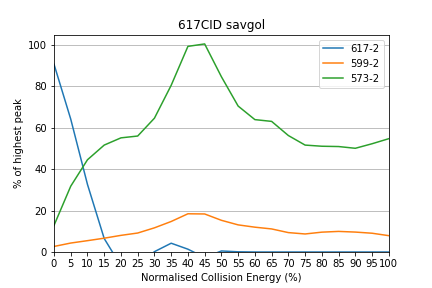
\includegraphics[width=\textwidth]{content/Anhang/ESIMS/Bo-DYCC/617CID-617-2savgol.png}
    \caption{}
  \end{subfigure}
  \hfill
  \begin{subfigure}[b]{0.5\textwidth}
    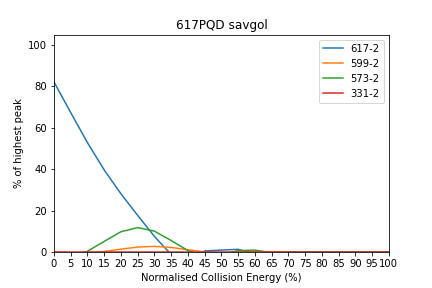
\includegraphics[width=\textwidth]{content/Anhang/ESIMS/Bo-DYCC/617PQD-617-2savgol.png}
    \caption{}
  \end{subfigure}
  
  \begin{subfigure}[b]{0.5\textwidth}
    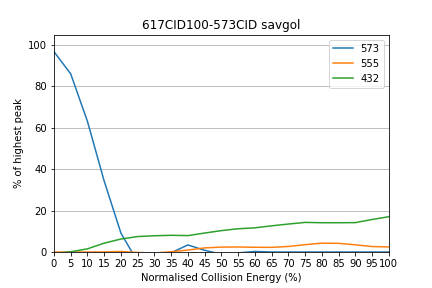
\includegraphics[width=\textwidth]{content/Anhang/ESIMS/Bo-DYCC/617CID100-573CID-573savgol.png}
    \caption{}
  \end{subfigure}
  
  \caption[Fragmentierungsdiagramme des \textit{Bo}-DYCC, Quelle: Autor]{Fragmentierungsdiagramme des \textit{Bo}-DYCC: (a) m/z = 617 [M+H]\textsuperscript{+} im CID Modus, (b) m/z = 617 [M+H]\textsuperscript{+} im PQD Modus, (c) (m/z)\textsuperscript{2} = 573 [M+H]\textsuperscript{+} im CID Modus}
\end{figure}

\pagebreak
\section{Bo-DNCC}

\begin{figure}[!htbp]
  \begin{subfigure}[b]{0.5\textwidth}
    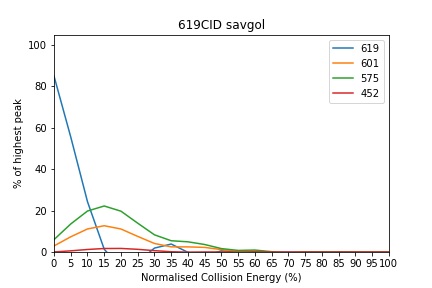
\includegraphics[width=\textwidth]{content/Anhang/ESIMS/Bo-DNCC/619CID-619savgol.png}
    \caption{}
  \end{subfigure}
  \hfill
  \begin{subfigure}[b]{0.5\textwidth}
    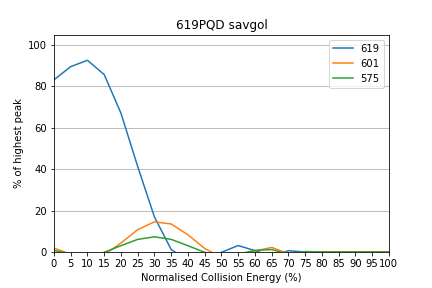
\includegraphics[width=\textwidth]{content/Anhang/ESIMS/Bo-DNCC/619PQD-619savgol.png}
    \caption{}
  \end{subfigure}
  
  \begin{subfigure}[b]{0.5\textwidth}
    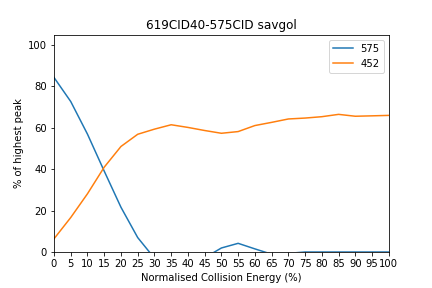
\includegraphics[width=\textwidth]{content/Anhang/ESIMS/Bo-DNCC/619CID40-575CID-575savgol.png}
    \caption{}
  \end{subfigure}
  \hfill
  \begin{subfigure}[b]{0.5\textwidth}
    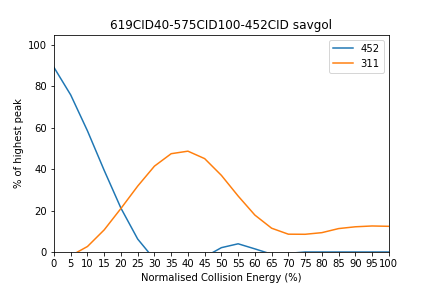
\includegraphics[width=\textwidth]{content/Anhang/ESIMS/Bo-DNCC/619CID40-575CID100-452CID-452savgol.png}
    \caption{}
  \end{subfigure}
  
  \caption[Fragmentierungsdiagramme des \textit{Bo}-DNCC, Quelle: Autor]{Fragmentierungsdiagramme des \textit{Bo}-DNCC: (a) m/z = 619 [M+H]\textsuperscript{+} im CID Modus, (b) m/z = 619 [M+H]\textsuperscript{+} im PQD Modus, (c) (m/z)\textsuperscript{2} = 575 [M+H]\textsuperscript{+} im CID Modus, (d) (m/z)\textsuperscript{3} = 452 [M+H]\textsuperscript{+} im CID Modus }
\end{figure}

\pagebreak
\section{Bo-NCC-1}

\begin{figure}[!htbp]
  \begin{subfigure}[b]{0.5\textwidth}
    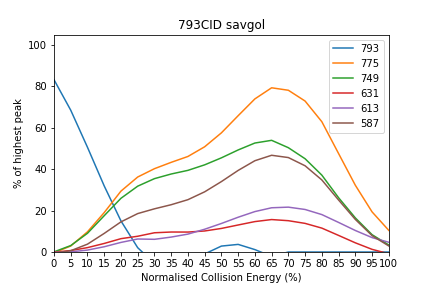
\includegraphics[width=\textwidth]{content/Anhang/ESIMS/Bo-NCC-1/793CID-793savgol.png}
    \caption{}
  \end{subfigure}
  \hfill
  \begin{subfigure}[b]{0.5\textwidth}
    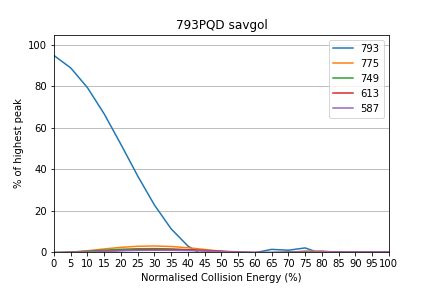
\includegraphics[width=\textwidth]{content/Anhang/ESIMS/Bo-NCC-1/793PQD-793savgol.png}
    \caption{}
  \end{subfigure}
  
  \begin{subfigure}[b]{0.5\textwidth}
    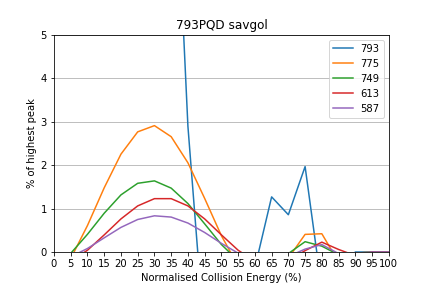
\includegraphics[width=\textwidth]{content/Anhang/ESIMS/Bo-NCC-1/793PQD-793savgolv5.png}
    \caption{}
  \end{subfigure}
  
  \caption[Fragmentierungsdiagramme des \textit{Bo}-NCC-1, Quelle: Autor]{Fragmentierungsdiagramme des \textit{Bo}-NCC-1: (a) m/z = 793 [M+H]\textsuperscript{+} im CID Modus, (b) m/z = 793 [M+H]\textsuperscript{+} im PQD Modus, (c) Ausschnitt aus Diagramm (b)}
\end{figure}

\pagebreak
\section{Bo-NCC-3}

\begin{figure}[!htbp]
  \begin{subfigure}[b]{0.5\textwidth}
    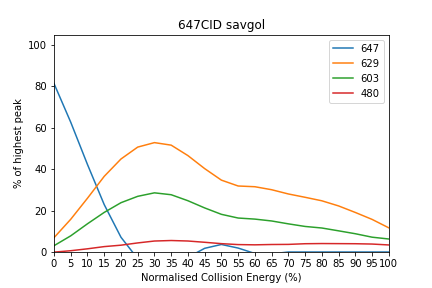
\includegraphics[width=\textwidth]{content/Anhang/ESIMS/Bo-NCC-3/647CID-647savgol.png}
    \caption{}
  \end{subfigure}
  \hfill
  \begin{subfigure}[b]{0.5\textwidth}
    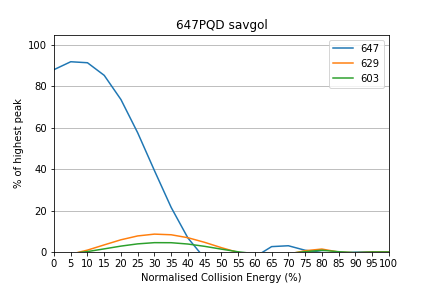
\includegraphics[width=\textwidth]{content/Anhang/ESIMS/Bo-NCC-3/647PQD-647savgol.png}
    \caption{}
  \end{subfigure}
  
  \caption[Fragmentierungsdiagramme des \textit{Bo}-NCC-3, Quelle: Autor]{Fragmentierungsdiagramme des \textit{Bo}-NCC-3: (a) m/z = 647 [M+H]\textsuperscript{+} im CID Modus, (b) m/z = 647 [M+H]\textsuperscript{+} im PQD Modus}
\end{figure}

\section{Reaktionsprodukt des Bo-DYCC}

\begin{figure}[!htbp]
  \begin{subfigure}[b]{0.5\textwidth}
    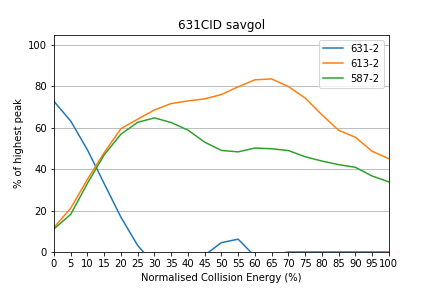
\includegraphics[width=\textwidth]{content/Anhang/ESIMS/RP_Bo-DYCC/631CID-631-2savgol.png}
    \caption{}
  \end{subfigure}
  \hfill
  \begin{subfigure}[b]{0.5\textwidth}
    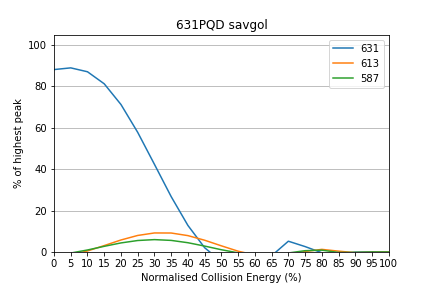
\includegraphics[width=\textwidth]{content/Anhang/ESIMS/RP_Bo-DYCC/631PQD-631savgol.png}
    \caption{}
  \end{subfigure}
  
  \caption[Fragmentierungsdiagramme des Reaktionsproduktes des \textit{Bo}-DYCC, Quelle: Autor]{Fragmentierungsdiagramme des Reaktionsproduktes des \textit{Bo}-DYCC: (a) m/z = 631 [M+H]\textsuperscript{+} im CID Modus, (b) m/z = 631 [M+H]\textsuperscript{+} im PQD Modus}
\end{figure}

\pagebreak
\section{Reaktionsprodukt des Bo-DNCC}

\begin{figure}[!htbp]
  \begin{subfigure}[b]{0.5\textwidth}
    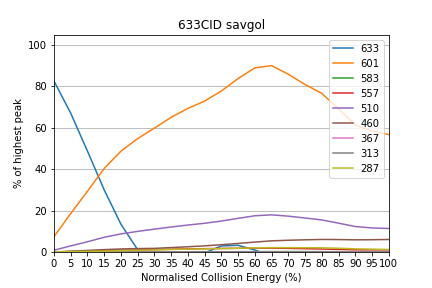
\includegraphics[width=\textwidth]{content/Anhang/ESIMS/RP_Bo-DNCC/633CID-633savgol.png}
    \caption{}
  \end{subfigure}
  \hfill
  \begin{subfigure}[b]{0.5\textwidth}
    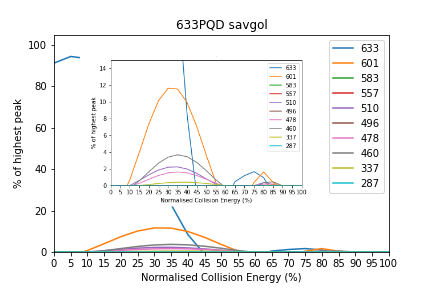
\includegraphics[width=\textwidth]{content/Anhang/ESIMS/RP_Bo-DNCC/633PQD-633savgol_pic.png}
    \caption{}
  \end{subfigure}
  
  \begin{subfigure}[b]{0.5\textwidth}
    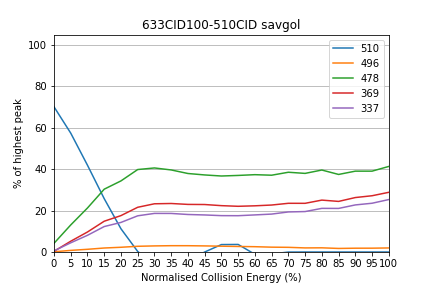
\includegraphics[width=\textwidth]{content/Anhang/ESIMS/RP_Bo-DNCC/633CID100-510CID-510savgol.png}
    \caption{}
  \end{subfigure}
  \hfill
  \begin{subfigure}[b]{0.5\textwidth}
    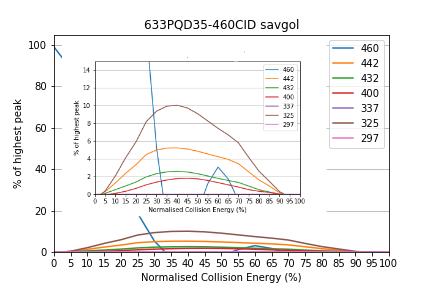
\includegraphics[width=\textwidth]{content/Anhang/ESIMS/RP_Bo-DNCC/633PQD35-460CID-460savgol_pic.png}
    \caption{}
  \end{subfigure}
  
  \begin{subfigure}[b]{0.5\textwidth}
    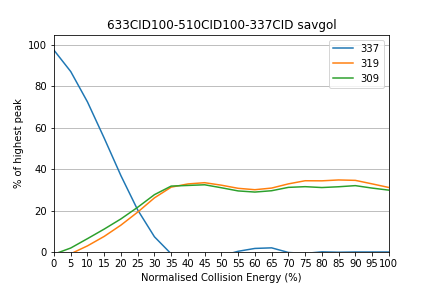
\includegraphics[width=\textwidth]{content/Anhang/ESIMS/RP_Bo-DNCC/633CID100-510CID100-337CID-337savgol.png}
    \caption{}
  \end{subfigure}
  
  \caption[Fragmentierungsdiagramme des Reaktionsproduktes des \textit{Bo}-DNCC, Quelle: Autor]{Fragmentierungsdiagramme des Reaktionsproduktes des \textit{Bo}-DNCC: (a) m/z = 633 [M+H]\textsuperscript{+} im CID Modus, (b) m/z = 633 [M+H]\textsuperscript{+} im PQD Modus, (c) (m/z)\textsuperscript{2} = 510 [M+H]\textsuperscript{+} im CID Modus, (d) (m/z)\textsuperscript{2} = 460 [M+H]\textsuperscript{+} im PQD Modus, (e) (m/z)\textsuperscript{3} = 337 [M+H]\textsuperscript{+} im CID Modus}
\end{figure}

\pagebreak
\section{Reaktionsprodukt des Bo-NCC-3}

\begin{figure}[!htbp]
  \begin{subfigure}[b]{0.5\textwidth}
    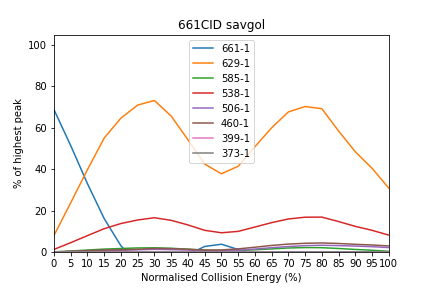
\includegraphics[width=\textwidth]{content/Anhang/ESIMS/RP_Bo-NCC-3/661CID-661-1savgol.png}
    \caption{}
  \end{subfigure}
  \hfill
  \begin{subfigure}[b]{0.5\textwidth}
    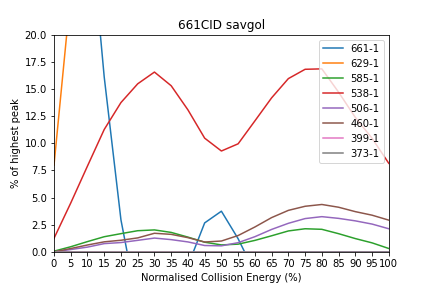
\includegraphics[width=\textwidth]{content/Anhang/ESIMS/RP_Bo-NCC-3/661CID-661-1savgolv20.png}
    \caption{}
  \end{subfigure}
  
  \begin{subfigure}[b]{0.5\textwidth}
    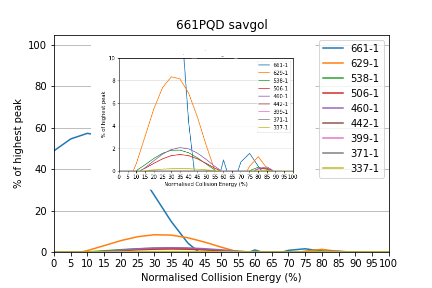
\includegraphics[width=\textwidth]{content/Anhang/ESIMS/RP_Bo-NCC-3/661PQD-661-1savgol_pic.png}
    \caption{}
  \end{subfigure}
  \hfill
  \begin{subfigure}[b]{0.5\textwidth}
    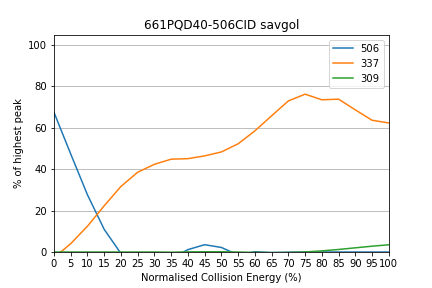
\includegraphics[width=\textwidth]{content/Anhang/ESIMS/RP_Bo-NCC-3/661PQD40-506CID-506savgol.png}
    \caption{}
  \end{subfigure}
  
  \begin{subfigure}[b]{0.5\textwidth}
    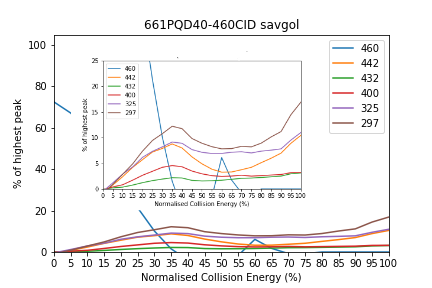
\includegraphics[width=\textwidth]{content/Anhang/ESIMS/RP_Bo-NCC-3/661PQD40-460CID-460savgol_pic.png}
    \caption{}
  \end{subfigure}
  \hfill
  \begin{subfigure}[b]{0.5\textwidth}
    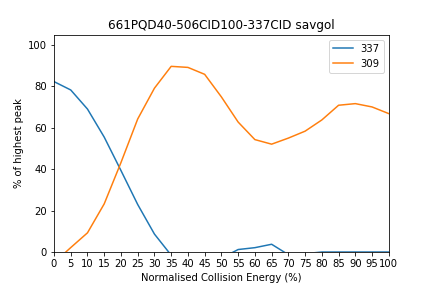
\includegraphics[width=\textwidth]{content/Anhang/ESIMS/RP_Bo-NCC-3/661PQD40-506CID100-337CID-337savgol.png}
    \caption{}
  \end{subfigure}
  
  \caption[Fragmentierungsdiagramme des Reaktionsproduktes des \textit{Bo}-NCC-3, Quelle: Autor]{Fragmentierungsdiagramme des Reaktionsproduktes des \textit{Bo}-NCC-3: (a) m/z = 661 [M+H]\textsuperscript{+} im CID Modus, (b) Ausschnitt aus Diagramm (a), (c) m/z = 661 [M+H]\textsuperscript{+} im PQD Modus, (d) (m/z)\textsuperscript{2} = 506 [M+H]\textsuperscript{+} im CID Modus, (e) (m/z)\textsuperscript{2} = 460 [M+H]\textsuperscript{+} im CID Modus, (f) (m/z)\textsuperscript{3} = 337 [M+H]\textsuperscript{+} im CID Modus}
\end{figure}
